\chapter{結論與未來展望}

\section{結論}
本論文提出了四項措施去改進第一版i18n工具所面臨的問題,分別是擴充代理關鍵字、支援所有html屬性的XPath翻譯邏輯、支援自由選擇翻譯的一詞多譯圖形化使用者介面、可以提供安裝的Python模組。透過以上努力,即可讓使用此i18n工具的多國語言網頁自動化驗收測試腳本,不再侷限於只能使用特定的關鍵字去撰寫。並且XPath的撰寫也不再需要考慮只有@title,text(),normalize-space()會被翻譯的問題,使用者的測試腳本可以用更多元的XPath寫法來搭配此i18n工具使用。遭遇一詞多譯時,使用者也能夠在第一次測試腳本結束後,選擇內心所預期的翻譯詞來執行接下來的測試。最後,藉由將i18n工具包裝成可以pip install 的Python模組,使用者可以隨安裝即使用本工具所提供的功能,而無須將自己的測試腳本移動到i18n工具的資料夾下。

\section{論文限制與未來展望}
本論文的i18n工具尚存在著使用限制,其原因之一源自於某些Robot Framework的原生關鍵字,其參數部分接受的是特殊的字元,目前i18n工具是不支援的。如圖5.1,Get Match Count接受的第二個參數是S*,用來抓出串列中符合的字串,若是強行將S*翻譯,便會直接導致測試結果出錯。

\begin{figure}[H]
\centering
\begin{lstlisting}[language={python}]
*** Test Cases ***
Get match count
    @{list1} =    Create List   Support    Software    Apple
    ${count} =    Get Match Count    ${list1}    S*
    Log    ${count} 
\end{lstlisting}
\caption{Get Match Count測試腳本}
\end{figure}

此外,某些Robot Framework的關鍵字,其內部實作會呼叫另一個原生的關鍵字,且被呼叫的關鍵字也有一詞多譯的需求。當使用者為第一次執行測試的一詞多譯選擇了翻譯後,並執行第二次測試腳本時,因為此時傳入代理關鍵字的參數部分已改變,系統會將其判定為不同的待翻譯詞,而需要使用者事後再選擇一次。如圖5.2 ,Dictionary Should Contain Item原生關鍵字的實作會呼叫Dictionary Should Contain Key(如圖5.3紅色框起部分),導致第一次執行測試時傳入的”More”,和第二次執行時傳入的”More”,由於參數紀錄的局部從[‘支援’, ‘支援服務’]變成[‘支援’],因此被系統判定成不同的待翻譯詞,需要重新選擇(如圖5.4)。\\

\begin{figure}[H]
\centering
\begin{lstlisting}[language={python}]
*** Test Cases ***
Dictionary should contain item
    &{dict1} =    Create Dictionary    More=Support
    Dictionary Should Contain Item    ${dict1}    More    Support
\end{lstlisting}
\caption{Dictioanry Should Contain Item測試腳本}
\end{figure}

\begin{figure}[H]
\centering
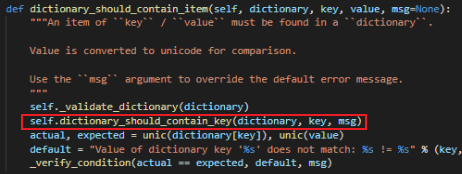
\includegraphics[width= \textwidth]{../論文截圖/5-1-2 dictionary should contain item測試腳本與其原生實作.png}
\caption{Dictioanry Should Contain Item原生實作}
\end{figure}

\begin{figure}[H]
\centering
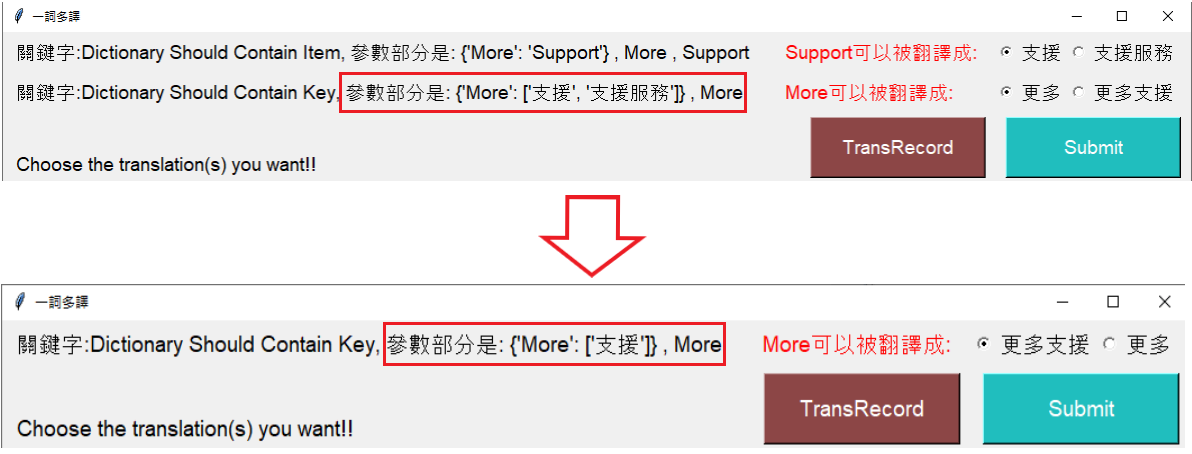
\includegraphics[width= \textwidth]{../論文截圖/5-1-3 1st&2nd執行測試腳本,待翻譯詞的參數紀錄變化.png}
\caption{第一次與第二次執行測試腳本,待翻譯詞的參數紀錄變化}
\end{figure}

未來展望的部分,可以根據i18n工具尚存在的使用限制,未來朝向優化特殊字元的翻譯方式,以及改善重複翻譯詞的判定邏輯去努力。記錄翻譯詞的部分,目前也只有記錄關鍵字的參數,少數情況下可能會和其他的關鍵字發生重疊,未來可以將關鍵字名稱一併記錄下來,以提高處理一詞多譯時的精確性。進而讓「多國語言網頁自動化驗收測試」工具變得更貼近測試者的需要,錯誤率低且容易使用。
